\documentclass[conference]{IEEEtran}

% \IEEEoverridecommandlockouts
% Only use the line above if you need a funding footnote.

\usepackage{cite}
\usepackage{amsmath,amssymb,amsfonts}
\usepackage{algorithmic}
\usepackage{graphicx}
\usepackage{textcomp}
\usepackage{xcolor}
\usepackage{comment}
\usepackage{tikz}
\usetikzlibrary{shapes, arrows.meta, positioning}

\def\BibTeX{{\rm B\kern-.05em{\sc i\kern-.025em b}\kern-.08em
    T\kern-.1667em\lower.7ex\hbox{E}\kern-.125emX}}

\begin{document}

\title{Comparing Known-Map and Incremental Mapping Navigation for Autonomous Restaurant Service Robots}

\author{
\IEEEauthorblockN{
Pedro Ferreira\textsuperscript{1,2},
Catarina Fernandes\textsuperscript{1,2},
Leonor Baía\textsuperscript{1,2},
Gonçalo Leão\textsuperscript{1,3},
Luís Paulo Reis\textsuperscript{1,4},
Armando Sousa\textsuperscript{1,3}
}

\IEEEauthorblockA{
\textsuperscript{1}FEUP -- Faculty of Engineering, University of Porto, Portugal\\
\textsuperscript{2}FCUP -- Faculty of Sciences, University of Porto, Portugal\\
\textsuperscript{3}INESC TEC -- INESC Technology and Science, Portugal\\
\textsuperscript{4}LIACC -- Artificial Intelligence and Computer Science Laboratory, Portugal
}

\IEEEauthorblockA{
\{up202208344, up202307632, up202304808\}@edu.fe.up.pt,
\{goncalo.leao, lpreis, asousa\}@fe.up.pt
}
}

\maketitle



\begin{abstract}

Autonomous service robots in restaurants must operate efficiently in constrained indoor layouts while reacting to static obstacles, moving people, and multiple service requests. This paper presents a Webots-based simulation of an e-puck waiter robot designed to serve tables in a restaurant scenario. The study compares two navigation approaches with different levels of environmental knowledge. The first approach uses a predefined occupancy grid of the restaurant and applies the A-star algorithm for global path planning. The second approach starts without a prior map and incrementally builds an occupancy grid from LiDAR (Light Detection and Ranging) observations combined with odometry-based pose estimation. The system also includes a request-management component that supports different request-selection policies when multiple tables are waiting. The robot is evaluated in static and dynamic scenarios, where moving obstacles simulate people inside the restaurant. Performance is analysed using service-oriented metrics such as waiting time, return time, total completion time, success rate, and qualitative navigation robustness. The goal is to clarify how prior map knowledge affects the efficiency and reliability of autonomous indoor restaurant service.
\end{abstract}

\begin{IEEEkeywords}
Autonomous service robots, mobile robotics, restaurant environment, Webots, e-puck, A-star path planning, occupancy grid mapping, LiDAR, request management, dynamic obstacles.
\end{IEEEkeywords}



\section{Introduction}

Autonomous mobile robots are increasingly used in indoor service environments to support repetitive tasks such as object transport and customer assistance. Restaurants are a relevant example, since a waiter robot must move between a base station and several tables while avoiding narrow passages, static obstacles, and moving people.

This work addresses autonomous table service in a simulated restaurant environment. The robot receives table requests, selects which request to serve, navigates to the corresponding service area, performs a short service action, and returns to the base station. The main focus of the study is the effect of prior environmental knowledge on navigation performance. Additionally, the system includes request-selection policies, such as arrival order, estimated distance, and a hybrid criterion, to handle situations where multiple tables are waiting.

This work was guided by the following research question: how does prior environmental knowledge influence the efficiency and robustness of an autonomous service robot in static and dynamic restaurant scenarios? The hypothesis is that a known-map approach will provide more efficient and stable navigation, while incremental mapping will offer greater flexibility at the cost of higher uncertainty.

To investigate this question, a restaurant scenario was developed in Webots using an e-puck mobile robot. Two navigation approaches are compared: a predefined occupancy grid with A-star path planning, and an incremental occupancy grid built from LiDAR and odometry data. Performance is evaluated using waiting time, return time, total completion time, success rate, and qualitative navigation robustness.

The remainder of this paper is organized as follows. Section II reviews related work. Section III describes the methodological approach. Section IV presents the experimental evaluation and results. Finally, Section V summarizes the conclusions and discusses future work.



\section{Related work}

Restaurant service robots have been studied as a practical application of autonomous mobile robotics. Cheong et al. developed a robotic waiter system for casual dining restaurants, focusing on autonomous food delivery and docking at target tables \cite{cheong2016roboticwaiter}. Their work shows that restaurant service requires more than simple movement between points, since the robot must operate in constrained layouts and reach service locations accurately.

More recent work has explored service robots in real fast-food environments. Chen et al. proposed a non-contact food service robot that combines mapping, localization, and navigation to support restaurant delivery tasks \cite{chen2022noncontact}. While their work focuses on a deployed service robot, the present work uses simulation to compare how different levels of prior environmental knowledge affect navigation performance under controlled static and dynamic conditions.

The restaurant scenario has also been approached from a planning perspective. Mohseni-Kabir et al. formalized waiting tables as a robot planning problem, where multiple independent tasks are partially observable and evolve over time \cite{mohseni2021waiting}. This is related to the request-management component used in this work, where table requests may appear while the robot is already serving another table.

From a navigation perspective, this work builds on classical path planning and mapping methods. The known-map approach uses the A-star algorithm, originally introduced by Hart et al. as a heuristic method for minimum-cost path search \cite{hart1968astar}. The incremental mapping approach is based on occupancy grids, a representation introduced by Elfes for mobile robot perception, world modelling, and navigation \cite{elfes1989occupancy}. In contrast with previous works focused on complete service robot deployment or individual navigation methods, this paper evaluates these components together in a simulated restaurant service scenario, comparing known-map navigation with incremental occupancy-grid mapping.



\section{Methodological approach}

This section describes how the proposed restaurant service robot system was designed and implemented.


\subsection{Simulation Platform and Robot Configuration}

The system was implemented in Webots using the e-puck mobile robot as the
service platform. The robot is controlled by a supervisor controller that
implements the full service loop: request reception, navigation to a selected
table, simulated service, return to the base station, and metric logging. The
robot starts near the service counter, at approximately $(0,-0.38)$ m, and its
base position is represented in the controller as $(0,-0.39)$ m.

The simulated e-puck uses differential-drive actuation through the left and
right wheel motors. Wheel encoders are used for odometry, while a compass
provides heading correction. The robot is also equipped with the eight
standard proximity sensors and a 360-degree planar LiDAR with a maximum range
of 2 m. The proximity sensors and LiDAR are used both for local obstacle
detection and for emergency recovery behaviours when the planned path becomes
unsafe. A short calibration phase is executed at startup to estimate proximity
sensor baselines and the initial compass heading.

Communication between the robot and the request-management controller is
implemented through Webots emitter and receiver devices. Table requests are
sent to the robot as messages containing the table identifier and the request
timestamp. After completing the service action, the robot sends a completion
message back to the manager, which updates the pending-request state and logs
completion metrics.


\subsection{Restaurant Environment}

The environment represents a small restaurant with a service counter, six
tables, chairs, boundary walls, and decorative plants. The layout was modelled
as a constrained indoor navigation scenario in which the robot must move
through narrow passages and approach each table without colliding with nearby
furniture. The tables are identified as T1 to T6 and are placed at fixed
coordinates:
T1 $=(-0.432,-0.312)$,
T2 $=(-0.168,-0.120)$,
T3 $=(-0.408,0.204)$,
T4 $=(0.396,-0.252)$,
T5 $=(0.144,0.084)$, and
T6 $=(0.432,0.336)$ m.

For each table, the controller stores one central table position and four
additional reach points around it. These candidate points allow the navigation
module to select an accessible service position when the table centre itself is
occupied by the physical table geometry. A request is considered served when
the robot reaches the corresponding service area within a radius of 0.15 m.
The robot is considered to have returned to the base when it reaches the base
position within a radius of 0.05 m.


\subsection{Request Management}

Requests are generated by a separate supervisor controller. The manager keeps a
set of pending tables, turns on the corresponding table lamp when a request is
created, and turns it off when the robot reports completion. New requests are
sent at configurable time intervals. In the policy-comparison experiments
available in the repository, the first request was generated after 5 s and
subsequent requests were generated every 8--16 s, using fixed random seeds for
repeatability.

When the robot is idle, a new request is started immediately. When the robot is
already travelling, serving, or returning to base, the request is inserted into
a queue. Three queue-selection policies are supported. The FIFO policy selects
the oldest queued request. The nearest policy selects the queued table with the
smallest estimated distance from the current robot position. The hybrid policy
combines fairness and travel cost using
\begin{equation}
score_i = w_t\,wait_i - w_d\,dist_i,
\end{equation}
where $wait_i$ is the elapsed time since request creation and $dist_i$ is the
estimated distance from the robot to the closest service point of table $i$.
The implementation uses $w_t=1.0$ and $w_d=30.0$ as the default hybrid
configuration. The selected request is the one with the highest score, as
illustrated in Fig.~\ref{fig:hybrid_policy}.

\begin{figure}[htbp]
\centering
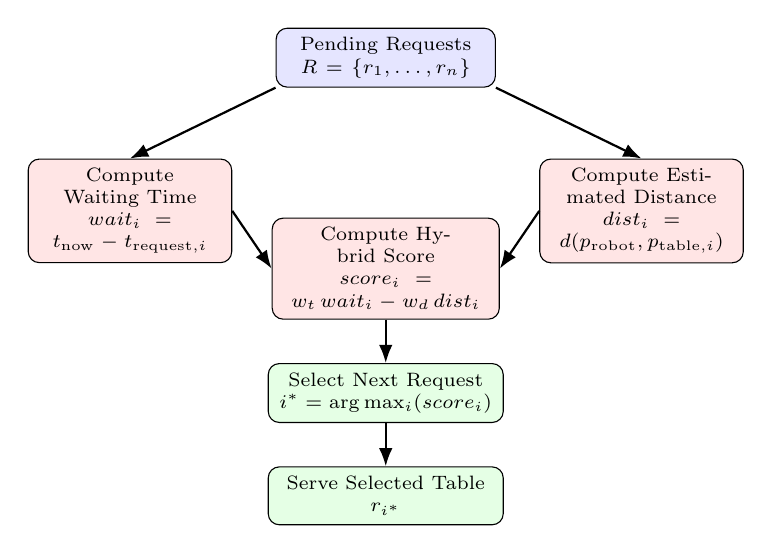
\begin{tikzpicture}[
    font=\scriptsize,
    node distance=0.55cm and 0.45cm,
    block/.style={
        draw,
        rounded corners,
        align=center,
        text width=2.55cm,
        minimum height=0.65cm,
        fill=blue!10
    },
    calc/.style={
        draw,
        rounded corners,
        align=center,
        text width=2.35cm,
        minimum height=0.9cm,
        fill=red!10
    },
    scorecalc/.style={
        draw,
        rounded corners,
        align=center,
        text width=2.65cm,
        minimum height=0.9cm,
        fill=red!10
    },
    output/.style={
        draw,
        rounded corners,
        align=center,
        text width=2.75cm,
        minimum height=0.72cm,
        fill=green!10
    },
    line/.style={draw, -Latex, thick}
]

\node[block] (pending)
{Pending Requests\\$R=\{r_1,\ldots,r_n\}$};

\node[calc, minimum height=1.1cm, below left=0.9cm and 0.55cm of pending] (wait)
{Compute Waiting Time\\$wait_i=t_{\mathrm{now}}-t_{\mathrm{request},i}$};

\node[calc, below right=0.9cm and 0.55cm of pending] (dist)
{Compute Estimated Distance\\$dist_i=d(p_{\mathrm{robot}},p_{\mathrm{table},i})$};

\node[scorecalc, below=1.65cm of pending] (score)
{Compute Hybrid Score\\$score_i=w_t\,wait_i-w_d\,dist_i$};

\node[output, below=0.55cm of score] (select)
{Select Next Request\\$i^*=\arg\max_i(score_i)$};

\node[output, below=0.55cm of select] (serve)
{Serve Selected Table\\$r_{i^*}$};

\draw[line] (pending.south west) -- (wait.north);
\draw[line] (pending.south east) -- (dist.north);

\draw[line] (wait.east) -- (score.west);
\draw[line] (dist.west) -- (score.east);

\draw[line] (score.south) -- (select.north);
\draw[line] (select.south) -- (serve.north);

\end{tikzpicture}
\caption{Hybrid request-selection policy combining waiting time and estimated distance.}
\label{fig:hybrid_policy}
\end{figure}


\subsection{Navigation Approaches}

Two navigation approaches were implemented to compare different levels of
prior environmental knowledge.

\subsubsection{Known-map navigation}

In the first approach, the robot uses a predefined occupancy grid representing
the restaurant. The grid has a resolution of 0.03 m per cell and covers a
rectangular area with origin $(-0.66,-0.57)$ m, width 44 cells, and height 38
cells. Walls, tables, the counter, and plants are inserted into the grid before
the experiment starts. Obstacles are inflated by one grid cell to account for
the robot footprint and to increase clearance from furniture.

For each service request, the robot converts its current world position and the
candidate table service points into grid coordinates. If a target candidate is
occupied, the closest free cell within a local search radius is used instead.
The global path is planned with A-star over the occupancy grid, allowing
8-connected movement. The planner evaluates all candidate service points and
keeps the shortest valid path. The resulting grid path is followed waypoint by
waypoint using heading control, with emergency obstacle recovery still
available if the local sensors detect an unsafe situation.

\subsubsection{Incremental mapping navigation}

In the second approach, the robot starts without a prior map. It maintains an
incremental occupancy grid of size $100 \times 100$ cells, with 0.03 m
resolution and origin $(-1.5,-1.5)$ m. Unknown cells are initialized with an
intermediate occupancy value, while LiDAR observations mark cells along each
ray as free and the ray endpoint as occupied when an obstacle is detected
within the LiDAR range. A Bresenham line traversal is used to update free cells
between the robot and each observed endpoint.

Before planning, occupied cells are inflated by two cells, corresponding to
approximately 0.06 m. The robot then runs A-star on the resulting planning grid
and replans every 2 s or whenever the target changes. Since the map is
incomplete during early navigation, the controller uses a fallback reactive
behaviour when no valid A-star path is available. This behaviour uses the
front, left, and right LiDAR sectors together with the proximity sensors to
slow down, steer away from obstacles, or execute a short recovery manoeuvre.
When the robot returns to the base in the incremental-mapping experiment, its
odometry estimate is reset to the known base position to reduce accumulated
pose drift between service missions.


\subsection{Dynamic Obstacles}

Dynamic obstacles are managed by a dedicated Webots supervisor controller. They
are represented by three moving cylindrical objects that simulate people or
temporary obstacles in the restaurant. The robot does not receive direct
information from this controller; it can only react to these obstacles through
its own LiDAR and proximity sensors.

The dynamic scenario is deterministic and repeats every 95 s. During the first
60 s, the three obstacles become active one at a time in consecutive 20 s
windows. Between 60 s and 85 s, all three obstacles are active simultaneously.
Between 85 s and 95 s, all dynamic obstacles are hidden below the floor. The
obstacles follow three predefined circuits: one along the upper corridor, one
around the central table area, and one near the base/counter region. At the end
of each cycle, the circuits rotate between obstacles so that the same object
does not always follow the same route.

\subsection{Experimental Protocol and Metrics}

Each service mission follows the same state sequence: idle, travelling to a
table, serving, and returning to base. The service action is simulated by
stopping the robot for 2 s at the selected table. During the experiments, the
controllers print structured metric lines that are later parsed into CSV files
by the analysis scripts. The recorded metrics include waiting time, delivery
time, return time, total completion time, success rate, mission time, travelled
distance, average speed, safety interventions, and pending-request waiting time
for requests that remain unserved when a run stops.

The existing policy-comparison runs use three random seeds, 1001--1003, and a
limit of 10 completed requests or 420 s of simulation time. The available
results compare FIFO, nearest, and hybrid request policies in the incremental
mapping mode and with dynamic obstacles disabled. These results are useful for
validating the request-management component, but they do not yet provide the
full comparison between known-map and incremental mapping navigation. Therefore,
the experimental evaluation should still include matched EXP1 and EXP2 runs
under the same request seeds and under both static and dynamic conditions.
Placeholders for these missing results are left in Section~IV.



\section{Experimental evaluation}

This section reports the available empirical results for the
request-selection component. The complete comparison between the known-map and
incremental mapping navigation approaches is still being consolidated and
should be evaluated with matched request sequences under both static and
dynamic conditions.

\subsection{Request-Selection Policy Experiment}

The request-selection policies were evaluated empirically by running the same
restaurant scenario multiple times with different queue-selection rules. The
experiment compared FIFO, nearest-first, and hybrid selection. The robot was
executed in the incremental mapping mode, with dynamic obstacles disabled, so
that the comparison focused on the effect of the request policy rather than on
external disturbances.

For each policy, three repetitions were executed using fixed random seeds
1001, 1002, and 1003. Each run stopped after 10 completed requests or after
420 s of simulation time. The first request was generated after 5 s, and
subsequent requests were generated at random intervals between 8 s and 16 s.
All runs used the same request-generation parameters, allowing the policies to
be compared under equivalent conditions.

The hybrid policy assigns a score to each pending request according to
\begin{equation}
score_i = w_t\,wait_i - w_d\,dist_i,
\end{equation}
where $wait_i$ is the time elapsed since the request was created and $dist_i$
is the estimated distance from the robot to the closest service point of table
$i$. In these experiments, the hybrid weights were set to $w_t=1.0$ and
$w_d=30.0$. Higher scores have higher priority.

These weights were selected empirically through a small parameter sweep. Since
waiting time is measured in seconds and distance is measured in metres, the
distance weight also acts as a scale factor between the two quantities. With
$w_t=1.0$ and $w_d=30.0$, one additional metre of travel is approximately
equivalent to 30 s of waiting time in the score. This scale is appropriate for
the restaurant layout because the estimated distances to pending tables are
usually in the range of approximately 0.1--0.8 m, producing distance penalties
of about 3--24 score units. Two short sweeps were performed: one tested
$w_t=1.0$ with $w_d \in \{25,30,35,40,50\}$, and another tested
$w_t \in \{1.0,1.5,2.0,3.0\}$ with $w_d \in \{20,30,40\}$. The configuration
$w_t=1.0$, $w_d=30.0$ was kept because it achieved one of the best
fairness-objective values among the tested hybrid configurations, with similar
results obtained for distance weights near 30--40.

The policies were ranked using a fairness-oriented objective. Completed
requests contribute their measured waiting time, while requests still pending
at the end of a run contribute their pending waiting time. This combined set is
called the effective waiting time. The objective is
\begin{equation}
J = \overline{W}_{\mathrm{eff}} + 0.25\,W_{\mathrm{eff}}^{\max},
\end{equation}
where $\overline{W}_{\mathrm{eff}}$ is the mean effective waiting time and
$W_{\mathrm{eff}}^{\max}$ is the maximum effective waiting time. Lower values
of $J$ indicate better performance. This criterion penalizes policies that
obtain low average waiting times by leaving some requests unattended for long
periods.

\begin{table}[htbp]
\caption{Request-selection policy comparison in the incremental mapping mode.}
\label{tab:policy_comparison}
\centering
\resizebox{\columnwidth}{!}{
\begin{tabular}{lrrrrrr}
\hline
Policy & $J$ & $\overline{W}_{\mathrm{eff}}$ & $W_{\mathrm{eff}}^{\max}$ & Mean wait & Pending & Mean return \\
\hline
NEAREST & 163.183 & 86.416 & 307.070 & 34.739 & 15 & 17.016 \\
HYBRID & 178.566 & 118.934 & 238.530 & 117.970 & 10 & 19.364 \\
FIFO & 189.288 & 123.040 & 264.990 & 127.060 & 10 & 21.515 \\
\hline
\end{tabular}
}
\end{table}

The nearest-first policy achieved the best value of the fairness objective and
the lowest mean waiting time for served requests. This indicates that, in the
tested layout, prioritizing the closest table substantially reduces travel
time and improves average service efficiency. However, nearest-first also left
the largest number of pending requests at the end of the runs, which suggests
a fairness limitation: nearby tables can be favoured repeatedly while more
distant requests remain waiting.

The hybrid policy did not outperform nearest-first in the global objective, but
it reduced the maximum effective waiting time from 307.070 s to 238.530 s.
This shows the intended compromise of the hybrid criterion: it sacrifices some
average efficiency in order to reduce extreme waiting times. FIFO had the
highest objective value and the highest mean waiting time among the three
policies, indicating that arrival order alone is less suitable when travel
costs differ significantly between tables.

Overall, the policy experiment suggests that nearest-first is the most
efficient policy for average service time in the current scenario, while the
hybrid policy is preferable when the objective is to reduce excessive waiting
for individual tables.

% TODO: Insert matched navigation results for EXP1 known-map navigation and
% EXP2 incremental mapping navigation. The comparison should use the same
% request seeds, request policy, maximum number of completed requests, and
% simulation time limit in both modes.

% TODO: Report static and dynamic-scenario results separately. Important
% metrics: success rate, mean/max waiting time, mean/max return time, mean/max
% total completion time, travelled distance, safety interventions, and
% qualitative failure modes such as blocked paths, oscillation, or excessive
% odometry drift.
\section{Conclusions and future work}



\begin{thebibliography}{00}

\bibitem{cheong2016roboticwaiter}
A. Cheong, M. W. S. Lau, E. Foo, J. Hedley, and J. W. Bo,
``Development of a robotic waiter system,''
\textit{IFAC-PapersOnLine}, vol. 49, no. 21, pp. 681--686, 2016.

\bibitem{chen2022noncontact}
C. S. Chen, C. J. Lin, and C. C. Lai,
``Non-contact service robot development in fast-food restaurants,''
\textit{IEEE Access}, vol. 10, pp. 31466--31479, 2022.

\bibitem{mohseni2021waiting}
A. Mohseni-Kabir, M. Veloso, and M. Likhachev,
``Waiting tables as a robot planning problem,''
\textit{arXiv preprint arXiv:2105.10133}, 2021.

\bibitem{hart1968astar}
P. E. Hart, N. J. Nilsson, and B. Raphael,
``A formal basis for the heuristic determination of minimum cost paths,''
\textit{IEEE Transactions on Systems Science and Cybernetics},
vol. 4, no. 2, pp. 100--107, 1968.

\bibitem{elfes1989occupancy}
A. Elfes,
``Using occupancy grids for mobile robot perception and navigation,''
\textit{Computer}, vol. 22, no. 6, pp. 46--57, 1989.

\end{thebibliography}

\begin{comment}
\begin{figure}[htbp]
\centering
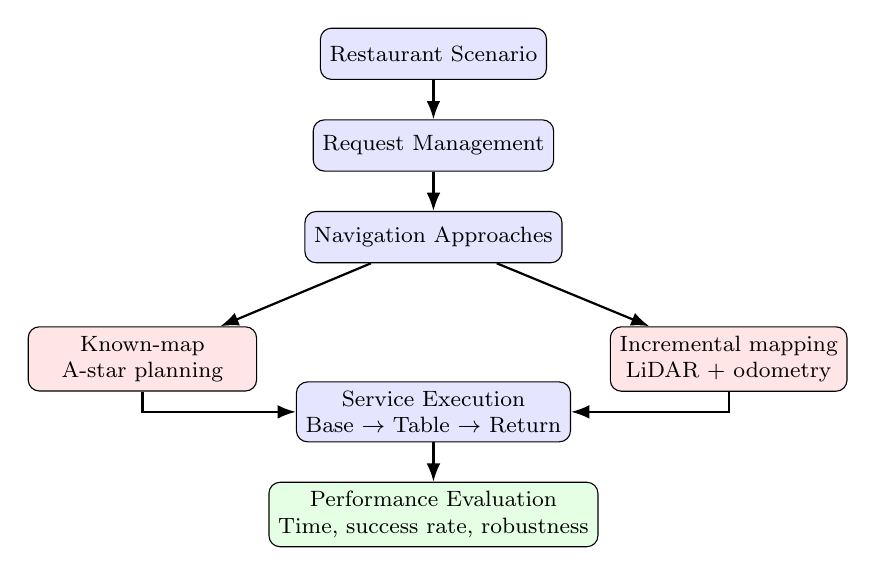
\begin{tikzpicture}[
    font=\footnotesize,
    node distance=0.5cm and 0.8cm,
    block/.style={
        draw,
        rounded corners,
        align=center,
        minimum width=2.8cm,
        minimum height=0.65cm,
        fill=blue!10
    },
    subblock/.style={
        draw,
        rounded corners,
        align=center,
        minimum width=2.9cm,
        minimum height=0.65cm,
        fill=red!10
    },
    output/.style={
        draw,
        rounded corners,
        align=center,
        minimum width=3.3cm,
        minimum height=0.7cm,
        fill=green!10
    },
    line/.style={draw, -Latex, thick}
]

\node[block] (env) {Restaurant Scenario};
\node[block, below=of env] (req) {Request Management};
\node[block, below=of req] (nav) {Navigation Approaches};

\node[subblock, below left=0.8cm and 0.6cm of nav] (known)
{Known-map\\A-star planning};

\node[subblock, below right=0.8cm and 0.6cm of nav] (inc)
{Incremental mapping\\LiDAR + odometry};

\node[block, below=1.5cm of nav] (exec)
{Service Execution\\Base $\rightarrow$ Table $\rightarrow$ Return};

\node[output, below=of exec] (eval)
{Performance Evaluation\\Time, success rate, robustness};

\draw[line] (env) -- (req);
\draw[line] (req) -- (nav);
\draw[line] (nav) -- (known);
\draw[line] (nav) -- (inc);
\draw[line] (known) |- (exec);
\draw[line] (inc) |- (exec);
\draw[line] (exec) -- (eval);

\end{tikzpicture}
\caption{Flowchart of the methodological approach.}
\label{fig:methodology}
\end{figure}
\end{comment}

\end{document}
